\definecolor{greenish}{RGB}{0,145,0}
\begin{tikzpicture}
	\pgfplotsset{/tikz/font={\small}}
	\begin{axis}[
			% title=Bitrate savings: $-8.94\%$. SNR improvement: $0.46$ dB,
			xlabel={ROM (kB)},
			ylabel={Y BD-rate (\%)},
			grid=both,
			scale only axis,
			width=0.9\textwidth,
			height=0.3\textheight,
			xtick={0.25,0.5,1,2,4,8,16,32,64,128,256,512,1024},
			xticklabels={0.25,0.5,1,2,4,8,16,32,64,128,256,512,1024},
			% x tick label style={
			% 	/pgf/number format/.cd,
			% 	fixed,
			% 	fixed zerofill,
			% 	precision=0,
			% },
			% scaled x ticks=false,
			ytick={0,-0.5,...,-4},
			y tick label style={
				/pgf/number format/.cd,
				fixed,
				fixed zerofill,
				precision=1,
				/tikz/.cd
			},
			xmode=log,
			log basis x=2,
			xmin=0.25, xmax=1024,
			ymin=-4.0, ymax=0,
			legend style={nodes=right},
			legend pos= south west
		]

		\addlegendentry{$4\times4$ non-sym. MDTC}
		\addplot [mark=x,mark size=2pt, red, thick, dashed,
		visualization depends on=\thisrow{alignment} \as \alignment,
		nodes near coords, % Place nodes near each coordinate
		point meta=explicit symbolic, % The meta data used in the nodes is not explicitly provided and not numeric
		every node near coord/.style={anchor=\alignment} % Align each coordinate at the anchor 40 degrees clockwise from the right edge
		] table [meta index=2] {
		rom	dtt_bdrate	dtt_label	alignment
		1.64	-0.49	\tiny{\color{black}4s1--8s0}	-90
		3.28	-0.67	\tiny{\color{black}4s2--8s0}	-90
		6.56	-0.82	\tiny{\color{black}4s4--8s0}	-90
		13.13	-0.93	\tiny{\color{black}4s8--8s0}	-90
		26.25	-0.98	\tiny{\color{black}4s16--8s0}	-90
		52.2	-1.01	\tiny{\color{black}4s32--8s0}	-90
		};

		\addlegendentry{$8\times8$ non-sym. MDTC}
		\addplot [mark=x,mark size=2pt, blue, thick, dashed,
		visualization depends on=\thisrow{alignment} \as \alignment,
		nodes near coords, % Place nodes near each coordinate
		point meta=explicit symbolic, % The meta data used in the nodes is not explicitly provided and not numeric
		every node near coord/.style={anchor=\alignment} % Align each coordinate at the anchor 40 degrees clockwise from the right edge
		] table [meta index=2] {
		rom	dtt_bdrate	dtt_label	alignment
		6.56	-0.84	\tiny{\color{black}4s0--8s1}	90
		13.13	-1.33	\tiny{\color{black}4s0--8s2}	90
		26.25	-1.72	\tiny{\color{black}4s0--8s4}	90
		52.50	-2.10	\tiny{\color{black}4s0--8s8}	90
		105.00	-2.48	\tiny{\color{black}4s0--8s16}	90
		210.00	-2.79	\tiny{\color{black}4s0--8s32}	90
		420.00	-3.07	\tiny{\color{black}4s0--8s64}	90
		840.00	-3.33	\tiny{\color{black}4s0--8s128}	45
		};

		% \addlegendentry{Comb. non-sym. MDTC}
		% \addplot [mark=x,mark size=2pt, greenish, thick, dashed,
		% visualization depends on=\thisrow{alignment} \as \alignment,
		% nodes near coords, % Place nodes near each coordinate
		% point meta=explicit symbolic, % The meta data used in the nodes is not explicitly provided and not numeric
		% every node near coord/.style={anchor=\alignment} % Align each coordinate at the anchor 40 degrees clockwise from the right edge
		% ] table [meta index=2] {
		% rom	dtt_bdrate	dtt_label	alignment
		% 8.20	-1.38	\tiny{\color{black}4s1--8s1}	180
		% 14.77	-1.80	\tiny{\color{black}4s1--8s2}	180
		% 16.41	-1.97	\tiny{\color{black}4s2--8s2}	180
		% 27.89	-2.14	\tiny{\color{black}4s1--8s4}	180
		% 32.81	-2.45	\tiny{\color{black}4s4--8s4}	180
		% 59.06	-2.76	\tiny{\color{black}4s4--8s8}	180
		% 65.62	-2.83	\tiny{\color{black}4s8--8s8}	180
		% 118.12	-3.15	\tiny{\color{black}4s8--8s16}	180
		% 223.12	-3.39	\tiny{\color{black}4s8--8s32}	-90
		% 236.25	-3.44	\tiny{\color{black}4s16--8s32}	90
		% };

		\addlegendentry{$4\times4$ sym. MDTC}
		\addplot [mark=*, mark size=1pt, red, thick,
		visualization depends on=\thisrow{alignment} \as \alignment,
		nodes near coords, % Place nodes near each coordinate
		point meta=explicit symbolic, % The meta data used in the nodes is not explicitly provided and not numeric
		every node near coord/.style={anchor=\alignment} % Align each coordinate at the anchor 40 degrees clockwise from the right edge
		] table [meta index=2] {
		rom	dtt_bdrate	dtt_label	alignment
		0.52	-0.50	\tiny{\color{black}4s1--8s0}	90
		1.03	-0.63	\tiny{\color{black}4s2--8s0}	-90
		2.06	-0.72	\tiny{\color{black}4s4--8s0}	90
		4.13	-0.84	\tiny{\color{black}4s8--8s0}	90
		8.25	-0.91	\tiny{\color{black}4s16--8s0}	90
		16.50	-0.93	\tiny{\color{black}4s32--8s0}	90
		};

		\addlegendentry{$8\times8$ sym. MDTC}
		\addplot [mark=*, mark size=1pt, blue, thick,
		visualization depends on=\thisrow{alignment} \as \alignment,
		nodes near coords, % Place nodes near each coordinate
		point meta=explicit symbolic, % The meta data used in the nodes is not explicitly provided and not numeric
		every node near coord/.style={anchor=\alignment} % Align each coordinate at the anchor 40 degrees clockwise from the right edge
		] table [meta index=2] {
		rom	dtt_bdrate	dtt_label	alignment
		2.06	-0.76	\tiny{\color{black}4s0--8s1}	0
		4.13	-1.24	\tiny{\color{black}4s0--8s2}	0
		8.25	-1.48	\tiny{\color{black}4s0--8s4}	0
		16.50	-1.97	\tiny{\color{black}4s0--8s8}	0
		% 33.00	    	\tiny{\color{black}4s0--8s16}	-90
		% 66.00	    	\tiny{\color{black}4s0--8s32}	-90
		% 132.00	   	\tiny{\color{black}4s0--8s64}	-90
		% 264.00	   	\tiny{\color{black}4s0--8s128}	-60
		};

		% \addlegendentry{Comb. sym. MDTC}
		% \addplot [mark=*, mark size=1pt, greenish, thick,
		% visualization depends on=\thisrow{alignment} \as \alignment,
		% nodes near coords, % Place nodes near each coordinate
		% point meta=explicit symbolic, % The meta data used in the nodes is not explicitly provided and not numeric
		% every node near coord/.style={anchor=\alignment} % Align each coordinate at the anchor 40 degrees clockwise from the right edge
		% ] table [meta index=2] {
		% rom	dtt_bdrate	dtt_label	alignment
		% 0.98	-0.74 \tiny{\color{black}1 kB}	0
		% 1.97	-1.02 \tiny{\color{black}2 kB}	0
		% 3.98	-1.39 \tiny{\color{black}4 kB}	0
		% 7.97	-1.82 \tiny{\color{black}8 kB}	0
		% 12.00	-2.10 \tiny{\color{black}12 kB}	0
		% 15.61	-2.22 \tiny{\color{black}16 kB}	0
		% 23.95	-2.52 \tiny{\color{black}24 kB}	0
		% 31.78	-2.68 \tiny{\color{black}32 kB}	0
		% 47.39	-2.85 \tiny{\color{black}48 kB}	0
		% 63.89	-3.00 \tiny{\color{black}64 kB}	0
		% 95.53	-3.27 \tiny{\color{black}96 kB}	0
		% 127.41	-3.41 \tiny{\color{black}128 kB}	0
		% };









\end{axis}
\end{tikzpicture}
